% Created by tikzDevice version 0.12 on 2019-02-08 11:01:12
% !TEX encoding = UTF-8 Unicode
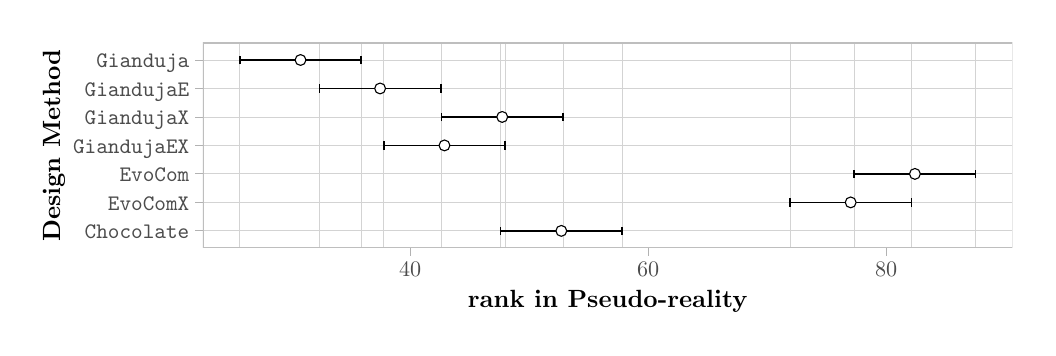
\begin{tikzpicture}[x=1pt,y=1pt]
\definecolor{fillColor}{RGB}{255,255,255}
\path[use as bounding box,fill=fillColor,fill opacity=0.00] (0,0) rectangle (361.35,108.41);
\begin{scope}
\path[clip] (  0.00,  0.00) rectangle (361.35,108.40);
\definecolor{drawColor}{RGB}{255,255,255}
\definecolor{fillColor}{RGB}{255,255,255}

\path[draw=drawColor,line width= 0.6pt,line join=round,line cap=round,fill=fillColor] (  0.00,  0.00) rectangle (361.35,108.40);
\end{scope}
\begin{scope}
\path[clip] ( 63.34, 28.81) rectangle (355.85,102.90);
\definecolor{fillColor}{RGB}{255,255,255}

\path[fill=fillColor] ( 63.34, 28.81) rectangle (355.85,102.90);
\definecolor{drawColor}{RGB}{211,211,211}

\path[draw=drawColor,line width= 0.3pt,line join=round] ( 63.34, 55.57) --
	(355.85, 55.57);

\path[draw=drawColor,line width= 0.3pt,line join=round] ( 63.34, 45.27) --
	(355.85, 45.27);

\path[draw=drawColor,line width= 0.3pt,line join=round] ( 63.34, 96.73) --
	(355.85, 96.73);

\path[draw=drawColor,line width= 0.3pt,line join=round] ( 63.34, 86.44) --
	(355.85, 86.44);

\path[draw=drawColor,line width= 0.3pt,line join=round] ( 63.34, 76.15) --
	(355.85, 76.15);

\path[draw=drawColor,line width= 0.3pt,line join=round] ( 63.34, 65.86) --
	(355.85, 65.86);

\path[draw=drawColor,line width= 0.3pt,line join=round] ( 63.34, 34.98) --
	(355.85, 34.98);

\path[draw=drawColor,line width= 0.2pt,line join=round] (214.79, 28.81) -- (214.79,102.90);

\path[draw=drawColor,line width= 0.2pt,line join=round] (342.55, 28.81) -- (342.55,102.90);

\path[draw=drawColor,line width= 0.2pt,line join=round] (319.34, 28.81) -- (319.34,102.90);

\path[draw=drawColor,line width= 0.2pt,line join=round] (120.55, 28.81) -- (120.55,102.90);

\path[draw=drawColor,line width= 0.2pt,line join=round] (149.30, 28.81) -- (149.30,102.90);

\path[draw=drawColor,line width= 0.2pt,line join=round] (172.56, 28.81) -- (172.56,102.90);

\path[draw=drawColor,line width= 0.2pt,line join=round] (193.43, 28.81) -- (193.43,102.90);

\path[draw=drawColor,line width= 0.2pt,line join=round] (170.88, 28.81) -- (170.88,102.90);

\path[draw=drawColor,line width= 0.2pt,line join=round] (298.65, 28.81) -- (298.65,102.90);

\path[draw=drawColor,line width= 0.2pt,line join=round] (275.43, 28.81) -- (275.43,102.90);

\path[draw=drawColor,line width= 0.2pt,line join=round] ( 76.64, 28.81) -- ( 76.64,102.90);

\path[draw=drawColor,line width= 0.2pt,line join=round] (105.39, 28.81) -- (105.39,102.90);

\path[draw=drawColor,line width= 0.2pt,line join=round] (128.66, 28.81) -- (128.66,102.90);

\path[draw=drawColor,line width= 0.2pt,line join=round] (149.53, 28.81) -- (149.53,102.90);
\definecolor{drawColor}{RGB}{0,0,0}

\path[draw=drawColor,line width= 0.6pt,line join=round] (214.79, 33.44) --
	(214.79, 36.53);

\path[draw=drawColor,line width= 0.6pt,line join=round] (214.79, 34.98) --
	(170.88, 34.98);

\path[draw=drawColor,line width= 0.6pt,line join=round] (170.88, 33.44) --
	(170.88, 36.53);

\path[draw=drawColor,line width= 0.6pt,line join=round] (342.55, 54.02) --
	(342.55, 57.11);

\path[draw=drawColor,line width= 0.6pt,line join=round] (342.55, 55.57) --
	(298.65, 55.57);

\path[draw=drawColor,line width= 0.6pt,line join=round] (298.65, 54.02) --
	(298.65, 57.11);

\path[draw=drawColor,line width= 0.6pt,line join=round] (319.34, 43.73) --
	(319.34, 46.82);

\path[draw=drawColor,line width= 0.6pt,line join=round] (319.34, 45.27) --
	(275.43, 45.27);

\path[draw=drawColor,line width= 0.6pt,line join=round] (275.43, 43.73) --
	(275.43, 46.82);

\path[draw=drawColor,line width= 0.6pt,line join=round] (120.55, 95.19) --
	(120.55, 98.27);

\path[draw=drawColor,line width= 0.6pt,line join=round] (120.55, 96.73) --
	( 76.64, 96.73);

\path[draw=drawColor,line width= 0.6pt,line join=round] ( 76.64, 95.19) --
	( 76.64, 98.27);

\path[draw=drawColor,line width= 0.6pt,line join=round] (149.30, 84.90) --
	(149.30, 87.98);

\path[draw=drawColor,line width= 0.6pt,line join=round] (149.30, 86.44) --
	(105.39, 86.44);

\path[draw=drawColor,line width= 0.6pt,line join=round] (105.39, 84.90) --
	(105.39, 87.98);

\path[draw=drawColor,line width= 0.6pt,line join=round] (172.56, 64.31) --
	(172.56, 67.40);

\path[draw=drawColor,line width= 0.6pt,line join=round] (172.56, 65.86) --
	(128.66, 65.86);

\path[draw=drawColor,line width= 0.6pt,line join=round] (128.66, 64.31) --
	(128.66, 67.40);

\path[draw=drawColor,line width= 0.6pt,line join=round] (193.43, 74.60) --
	(193.43, 77.69);

\path[draw=drawColor,line width= 0.6pt,line join=round] (193.43, 76.15) --
	(149.53, 76.15);

\path[draw=drawColor,line width= 0.6pt,line join=round] (149.53, 74.60) --
	(149.53, 77.69);

\path[draw=drawColor,line width= 0.4pt,line join=round,line cap=round,fill=fillColor] (192.83, 34.98) circle (  1.96);

\path[draw=drawColor,line width= 0.4pt,line join=round,line cap=round,fill=fillColor] (320.60, 55.57) circle (  1.96);

\path[draw=drawColor,line width= 0.4pt,line join=round,line cap=round,fill=fillColor] (297.39, 45.27) circle (  1.96);

\path[draw=drawColor,line width= 0.4pt,line join=round,line cap=round,fill=fillColor] ( 98.59, 96.73) circle (  1.96);

\path[draw=drawColor,line width= 0.4pt,line join=round,line cap=round,fill=fillColor] (127.35, 86.44) circle (  1.96);

\path[draw=drawColor,line width= 0.4pt,line join=round,line cap=round,fill=fillColor] (150.61, 65.86) circle (  1.96);

\path[draw=drawColor,line width= 0.4pt,line join=round,line cap=round,fill=fillColor] (171.48, 76.15) circle (  1.96);
\definecolor{drawColor}{RGB}{190,190,190}

\path[draw=drawColor,line width= 0.6pt,line join=round,line cap=round] ( 63.34, 28.81) rectangle (355.85,102.90);
\end{scope}
\begin{scope}
\path[clip] (  0.00,  0.00) rectangle (361.35,108.41);
\definecolor{drawColor}{gray}{0.30}

\node[text=drawColor,anchor=base east,inner sep=0pt, outer sep=0pt, scale=  0.80] at ( 58.39, 52.81) {\texttt{EvoCom}};

\node[text=drawColor,anchor=base east,inner sep=0pt, outer sep=0pt, scale=  0.80] at ( 58.39, 42.52) {\texttt{EvoComX}};

\node[text=drawColor,anchor=base east,inner sep=0pt, outer sep=0pt, scale=  0.80] at ( 58.39, 93.98) {\texttt{Gianduja}};

\node[text=drawColor,anchor=base east,inner sep=0pt, outer sep=0pt, scale=  0.80] at ( 58.39, 83.68) {\texttt{GiandujaE}};

\node[text=drawColor,anchor=base east,inner sep=0pt, outer sep=0pt, scale=  0.80] at ( 58.39, 73.39) {\texttt{GiandujaX}};

\node[text=drawColor,anchor=base east,inner sep=0pt, outer sep=0pt, scale=  0.80] at ( 58.39, 63.10) {\texttt{GiandujaEX}};

\node[text=drawColor,anchor=base east,inner sep=0pt, outer sep=0pt, scale=  0.80] at ( 58.39, 32.23) {\texttt{Chocolate}};
\end{scope}
\begin{scope}
\path[clip] (  0.00,  0.00) rectangle (361.35,108.41);
\definecolor{drawColor}{gray}{0.70}

\path[draw=drawColor,line width= 0.3pt,line join=round] ( 60.59, 55.57) --
	( 63.34, 55.57);

\path[draw=drawColor,line width= 0.3pt,line join=round] ( 60.59, 45.27) --
	( 63.34, 45.27);

\path[draw=drawColor,line width= 0.3pt,line join=round] ( 60.59, 96.73) --
	( 63.34, 96.73);

\path[draw=drawColor,line width= 0.3pt,line join=round] ( 60.59, 86.44) --
	( 63.34, 86.44);

\path[draw=drawColor,line width= 0.3pt,line join=round] ( 60.59, 76.15) --
	( 63.34, 76.15);

\path[draw=drawColor,line width= 0.3pt,line join=round] ( 60.59, 65.86) --
	( 63.34, 65.86);

\path[draw=drawColor,line width= 0.3pt,line join=round] ( 60.59, 34.98) --
	( 63.34, 34.98);
\end{scope}
\begin{scope}
\path[clip] (  0.00,  0.00) rectangle (361.35,108.41);
\definecolor{drawColor}{gray}{0.70}

\path[draw=drawColor,line width= 0.3pt,line join=round] (138.24, 26.06) --
	(138.24, 28.81);

\path[draw=drawColor,line width= 0.3pt,line join=round] (224.21, 26.06) --
	(224.21, 28.81);

\path[draw=drawColor,line width= 0.3pt,line join=round] (310.19, 26.06) --
	(310.19, 28.81);
\end{scope}
\begin{scope}
\path[clip] (  0.00,  0.00) rectangle (361.35,108.41);
\definecolor{drawColor}{gray}{0.30}

\node[text=drawColor,anchor=base,inner sep=0pt, outer sep=0pt, scale=  0.80] at (138.24, 18.35) {40};

\node[text=drawColor,anchor=base,inner sep=0pt, outer sep=0pt, scale=  0.80] at (224.21, 18.35) {60};

\node[text=drawColor,anchor=base,inner sep=0pt, outer sep=0pt, scale=  0.80] at (310.19, 18.35) {80};
\end{scope}
\begin{scope}
\path[clip] (  0.00,  0.00) rectangle (361.35,108.41);
\definecolor{drawColor}{RGB}{0,0,0}

\node[text=drawColor,anchor=base,inner sep=0pt, outer sep=0pt, scale=  0.90] at (209.60,  7.44) {\bfseries rank in Pseudo-reality};
\end{scope}
\begin{scope}
\path[clip] (  0.00,  0.00) rectangle (361.35,108.41);
\definecolor{drawColor}{RGB}{0,0,0}

\node[text=drawColor,rotate= 90.00,anchor=base,inner sep=0pt, outer sep=0pt, scale=  0.90] at ( 11.71, 65.86) {\bfseries Design Method};
\end{scope}
\end{tikzpicture}
